\documentclass{article}
% --- watermark (auto-inserted) ---
\usepackage{xcolor}
\usepackage{xfp}% \fpeval; in the kernel since 2022, harmless on older LaTeX
\usepackage{draftwatermark}
\newlength{\watermarkTextWidth}
\AddToHook{begindocument/end}{%
  \SetWatermarkText{\normalfont Generated by The Agentic Scientist}%
  \SetWatermarkFontSize{10pt}%
  \SetWatermarkLightness{0.85}%
  \settowidth{\watermarkTextWidth}{\normalfont\fontsize{10pt}{12pt}\selectfont Generated by The Agentic Scientist}%
  \edef\watermarkScale{\fpeval{0.8 * sqrt(\paperwidth**2 + \paperheight**2) / \watermarkTextWidth}}%
  \edef\watermarkAngle{\fpeval{atand(\paperheight/\paperwidth)}}%
  \SetWatermarkScale{\watermarkScale}%
  \SetWatermarkAngle{\watermarkAngle}%
}
% --- end watermark ---

\usepackage{iclr2026_conference,times}
\usepackage{amsmath,amssymb,booktabs,graphicx,subcaption}
\usepackage{hyperref,url}
\title{Scale-Adaptive Conformal Regions:\\Reliability and Limits on the Simplex}
\author{}
\newcommand{\R}{\mathbb{R}}
\newcommand{\simplex}{\Delta^{K-1}_{\circ}}
\newcommand{\clip}{\operatorname{clip}}
\begin{document}
\maketitle

\begin{abstract}
Prediction regions for compositional responses must account for both the simplex constraint and variation in predictive uncertainty. We study whether scale-adaptive split-conformal regions in isometric-logratio coordinates improve reliability and efficiency together. A frozen training-only procedure combines ridge centers, local residual-moment scaling, and nested rank-based selection; independent calibration determines the final regions. Across logistic-normal, Dirichlet, and shifted-Dirichlet settings at two dimensions and eight held-out seeds, the results are condition-dependent. Mean absolute coverage error is 0.0136 under IID sampling but 0.1303 under shift. Aggregate utility exceeds the strongest standard comparator by 0.0116, with a descriptive paired 95\% seed-bootstrap interval of [0.0047, 0.0179], yet mean uniform-simplex region mass is larger: 0.3035 versus 0.2917. Gains concentrate in higher-dimensional IID Dirichlet responses, whereas shifted comparisons favor the simplex-coordinate baseline. These findings support separating observed-response coverage, reference-measure efficiency, and distributional assumptions rather than interpreting an aggregate utility gain as uniform dominance or conditional validity.
% @evidence[[paper_data.json#/final_evaluation/metrics]]
% @evidence[[analysis/summary.json#/paired_overall/simplex_linf]]
\end{abstract}

\section{Introduction}
Compositional predictions arise whenever the response is a nonnegative vector constrained to sum to one. A region around such a prediction should respect the constraint, cover the relevant future observation, and remain informative. These requirements are distinct. A small region in transformed coordinates need not occupy little of the simplex; a marginally calibrated region need not be reliable within a feature-defined population; and reliable IID behavior need not persist after a change in covariate distribution. The target itself also matters: uncertainty for an observed continuous composition is not the same problem as a set of possible class labels or a confidence region for an unobserved probability vector.

Split conformal prediction supplies a natural starting point because its marginal coverage guarantee separates fitting a predictive score from calibrating its threshold \citep{Papadopoulos2002,Lei2018,Angelopoulos2021}. Compositional geometry nevertheless leaves important evaluation choices. Logratio representations remove the sum constraint but change how region size is measured \citep{Aitchison1982,Egozcue2003}. Heteroscedastic scaling can redistribute widths without altering the calibration rule. Consequently, judging a region construction requires more than a single coverage number or a single transformed-space volume.

We ask: \emph{how do training-only scale-adaptive logratio regions trade observed-composition coverage against uniform-simplex reference mass, relative to alternatives sharing the same fitted center?} We evaluate one fixed construction rather than claiming a comprehensive comparison of conformal methods. Its scale correction uses local moments of cross-fitted standardized residuals, with a neutral option and nested training-only selection. The final calibration sample is not used to choose that correction. The comparison includes unscaled logratio regions, a joint simplex-coordinate maximum-residual region, and coordinatewise Bonferroni regions.

The empirical answer is not uniform improvement. The scale-adaptive construction has higher aggregate utility but larger aggregate simplex mass than the simplex-coordinate baseline. The most favorable contrast occurs for IID Dirichlet responses in the larger dimension; shifted conditions provide clear adverse comparisons. Thus the useful contribution is a bounded evaluation of a specified configuration and its failure modes, not a new distribution-free guarantee. % @evidence[[analysis/summary.json]]

Our contributions are: (i) an inspectable training-only scale-adaptation specification with independent finite-rank calibration; (ii) a paired synthetic assessment separating coverage, reference mass, and their utility summary; and (iii) a seed-level uncertainty analysis that retains unfavorable condition-specific comparisons and distinguishes scaling effects from untested selector-specific explanations. The scope is strictly positive continuous responses under the stated generators. Structural zeros, latent probability recovery, real-data performance, and universal geometric preferences are outside the evidence.

\begin{figure}[t]
\centering
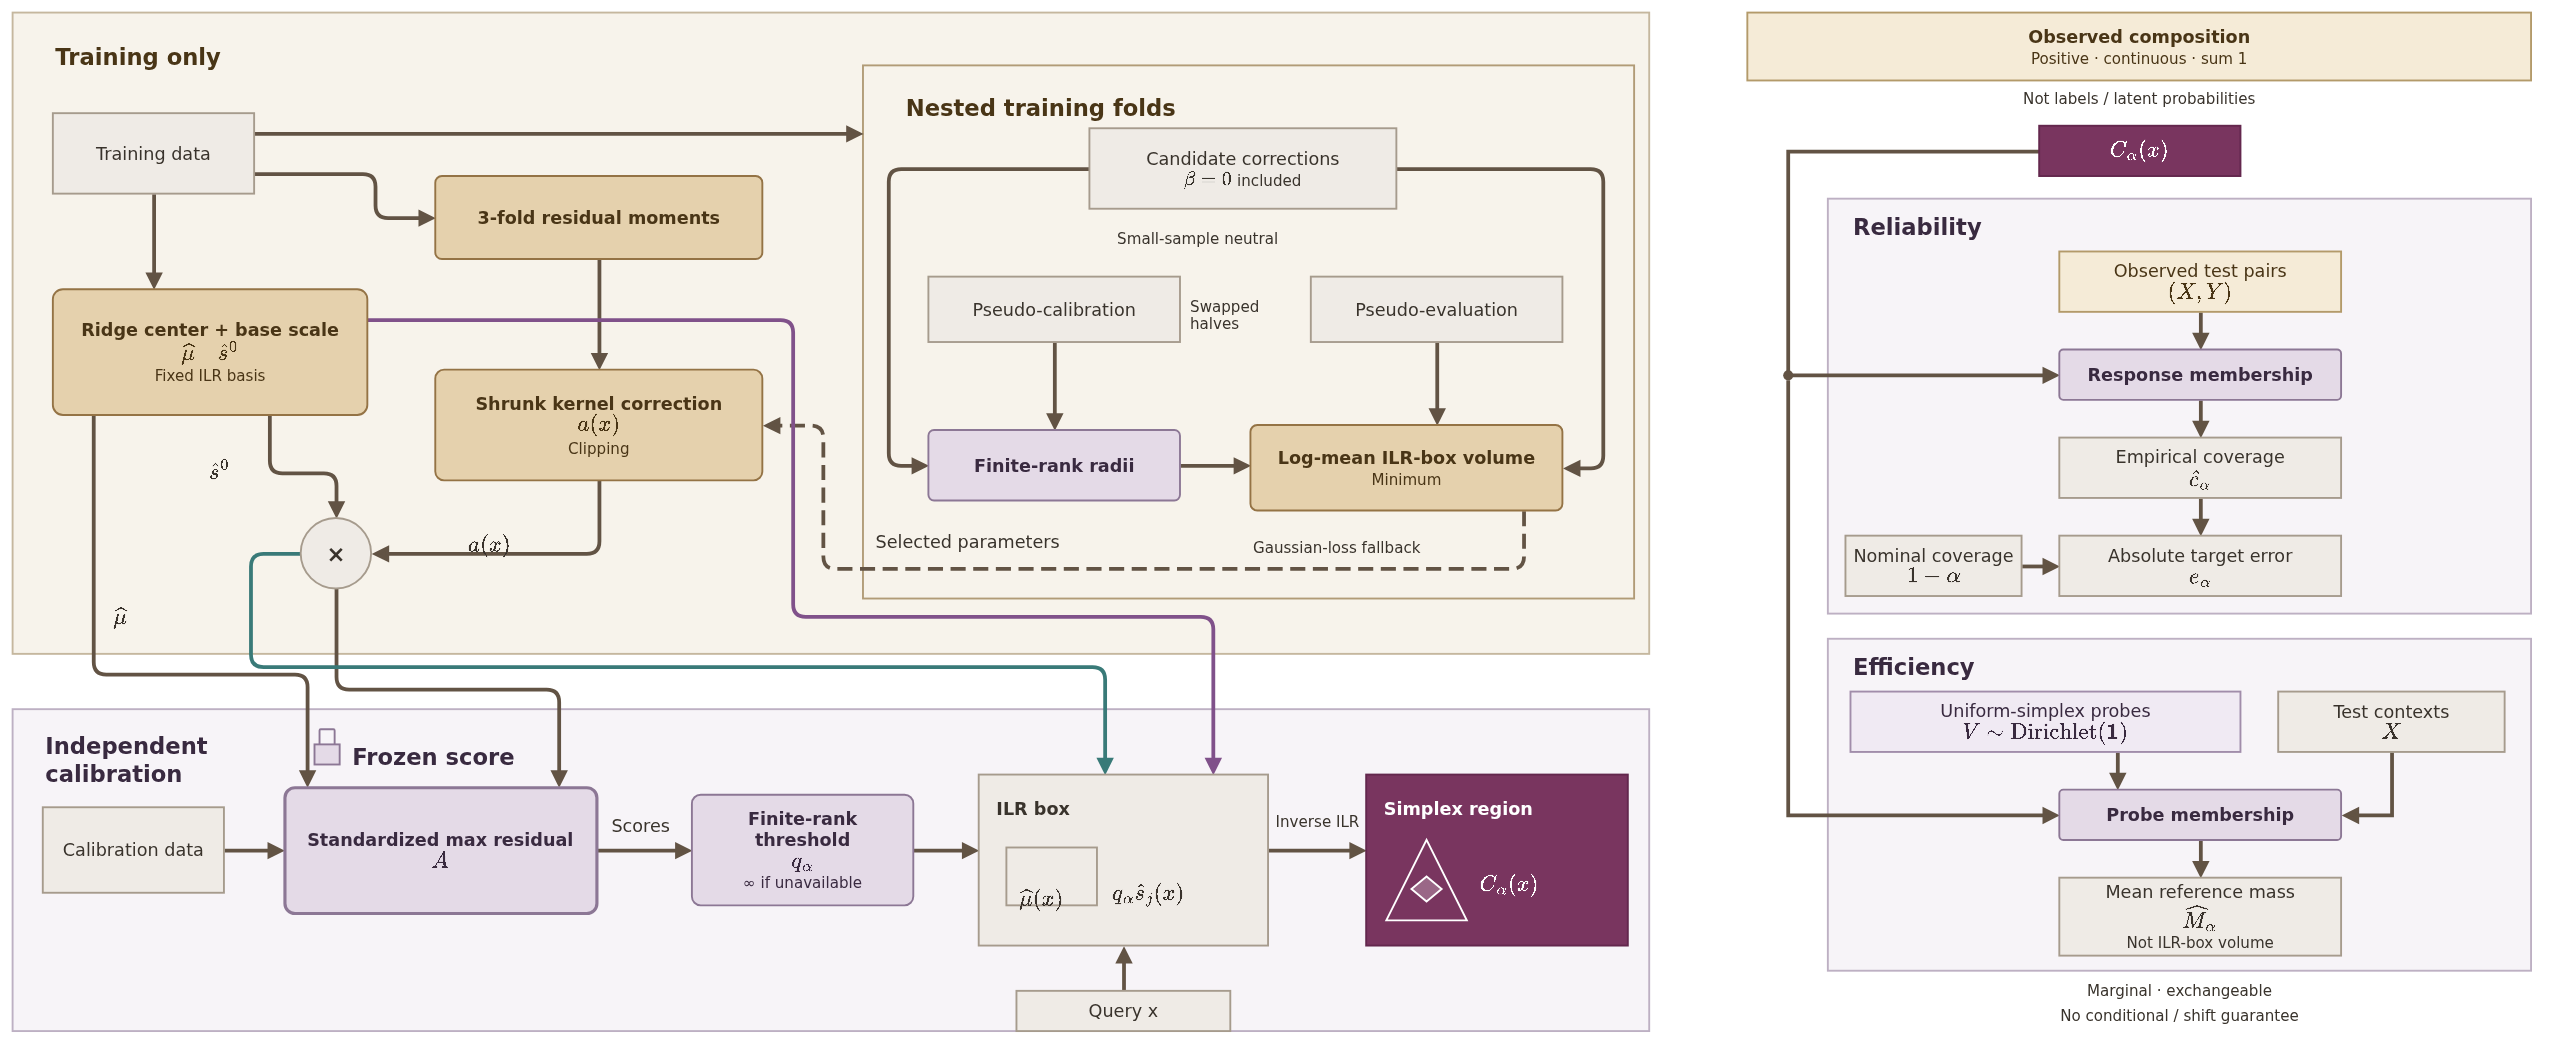
\includegraphics[width=.98\textwidth,height=1.6in,keepaspectratio]{figures/composition_reliability_overview.png}
\caption{Study overview. Training data determine centers and local scales, including internal rank-based selection. A separate calibration sample determines conformal thresholds. Evaluation distinguishes membership of observed compositions from mass under a uniform-simplex reference distribution; neither estimand establishes conditional or shifted validity.}
\label{fig:overview}
% @evidence[[source_evidence/selected_model.py]]
% @evidence[[source_evidence/evaluate_final.py]]
\end{figure}

\section{Related Work}
\paragraph{Calibration and adaptation.}
The conformal framework provides finite-sample predictive coverage under exchangeability \citep{Vovk2005}; inductive constructions separate model fitting and calibration \citep{Papadopoulos2002}. Regression studies compare the statistical and computational behavior of full and split conformal inference \citep{Lei2018}, while jackknife+ uses leave-one-out predictions to account for fitting variability \citep{Barber2021Jackknife}. Here the calibration procedure is ordinary split conformal: internal cross-fitting estimates scale information but is not jackknife+ calibration. Locally adaptive intervals have been developed through quantile regression \citep{Romano2019,Sesia2020}, conditional density estimation \citep{Lei2014,Izbicki2020}, and localized conformal constructions \citep{Guan2023}. These motivate adaptation without establishing that our particular scalar correction is optimal. Selection and aggregation raise a separate issue from calibrating one fixed score \citep{Yang2024}; our fitting choices are confined to training data.

\paragraph{What coverage does not imply.}
Conditional validity requires care even for inductive predictors \citep{Vovk2012}. Distribution-free conditional predictive inference has fundamental limits \citep{Barber2021Limits}, so pooled coverage should not be promoted to a feature-conditional guarantee. Under covariate shift, weighted conformal methods use covariate likelihood ratios \citep{Tibshirani2019}; broader departures from exchangeability require their own analysis \citep{Barber2023Beyond}. Adaptive conformal inference instead studies an online coverage-frequency target \citep{Gibbs2021}. These extensions are not implemented here. Our shifted evaluation is a stress test of a fixed, unweighted calibration rule, not a comparison with shift-aware methods.

\paragraph{Composition and statistical measurement.}
Compositional analysis treats ratios and the simplex as central objects \citep{Aitchison1982,Pawlowsky2015}; logistic-normal distributions provide transformed-normal models on that space \citep{Aitchison1980}. Isometric logratio (ILR) coordinates give an orthonormal representation \citep{Egozcue2003}, but orthonormality in logratio geometry does not preserve uniform-simplex mass. Our centers use ridge regression \citep{Hoerl1970}, and the scale correction is a shrunk kernel regression of residual moments in the spirit of \citet{Nadaraya1964}. Uncertainty reporting uses resampling across independent seed blocks \citep{Efron1979,Davison1997} and distinguishes those intervals from within-sample Wilson coverage intervals \citep{Brown2001}. The contribution is the resulting controlled audit, not a claim to originate any of these ingredients.

\section{Prediction Regions and Evaluation Targets}
\label{sec:regions}
\subsection{Problem setup and calibration}
Let $X\in\R^6$ and $Y\in\simplex=\{y\in(0,1)^K:\sum_k y_k=1\}$. We predict a region $C_\alpha(X)$ for an independent \emph{observed response} $Y$, at target coverage $1-\alpha$. No class label or latent multinomial parameter is evaluated. A fixed Helmert matrix $B\in\R^{K\times(K-1)}$ satisfies $B^\top B=I$ and $B^\top\mathbf 1=0$; the representation is
\begin{equation}
 z(y)=B^\top\log y,\qquad h(z)=\operatorname{softmax}(Bz).
\end{equation}
Fitted center $\widehat\mu(x)\in\R^{K-1}$ and positive scales $\widehat s_j(x)$ define the nonconformity score
\begin{equation}
 A(x,y)=\max_{1\leq j<K}\frac{|z_j(y)-\widehat\mu_j(x)|}{\widehat s_j(x)}.
 \label{eq:score}
\end{equation}
% @evidence[[source_evidence/selected_model.py#_basis]]
% @evidence[[source_evidence/evaluate_final.py#method_records]]
Given $m$ independent calibration scores, use the $r$th smallest score with $r=\lceil(m+1)(1-\alpha)\rceil$, or $+\infty$ if $r>m$. The region consists of positive compositions satisfying $A(x,y)\leq q_\alpha$. It is an axis-aligned box in the fixed ILR basis, mapped back to the simplex; it is not a full-covariance ellipsoid. The finite-rank rule, including its infinite-threshold case, is owned by the evaluation code rather than the fitted predictor. % @evidence[[source_evidence/evaluate_final.py#quantile]]

Conditional on the training data, exchangeable calibration and test scores give $\Pr\{Y\in C_\alpha(X)\}\geq1-\alpha$ by the standard conformal rank argument \citep{Lei2018}. Ties are handled conservatively by the non-strict membership inequality. This is a statement about a random calibration sample and future response, not a guarantee for every realized test set, every fixed feature vector, or every group. Training-only adaptation leaves this argument intact because the final calibration responses do not enter score selection. The argument does not apply unchanged to our shifted test sample.

\subsection{Reliability, mass, and utility}
For each fitted instance, empirical coverage $\widehat c_\alpha$ is the fraction of test responses inside the region. Reliability error is $e_\alpha=|\widehat c_\alpha-(1-\alpha)|$, treating overcoverage and undercoverage symmetrically. Efficiency is the normalized uniform-simplex reference mass
\begin{equation}
 M_\alpha=\mathbb E_{X_{\rm test}}\Pr_{V\sim\operatorname{Dirichlet}(\mathbf1)}
 \{V\in C_\alpha(X_{\rm test})\}.
 \label{eq:mass}
\end{equation}
The implementation estimates this probability with shared probes and test contexts, not by integrating ILR-box volume. Thus $M_\alpha\in[0,1]$ is dimension-normalized simplex volume, not probability content under the response law. We use ``mass'' to keep the reference distribution explicit. Small mass alone does not establish informative calibrated prediction. % @evidence[[source_evidence/evaluate_final.py#generate_arrays]]

The supplied utility combines the two empirical quantities:
\begin{equation}
 U_\alpha=(1-\widehat M_\alpha)
 \max\left\{0,1-\frac{e_\alpha}{1-\alpha}\right\}.
 \label{eq:utility}
\end{equation}
It rewards small regions and penalizes coverage error but is not a coverage constraint. A method can improve $U_\alpha$ by trading mass against error; its ordering need not agree with either component. We therefore report all components and treat utility as a supplied descriptive summary, not a proof of scientific superiority. Overall utility averages conditions and nominal levels equally. IID and shifted errors are averaged separately, after taking absolute deviations within each seed, condition, and level. Taking the absolute value after averaging coverage would produce a different estimand. % @evidence[[source_evidence/evaluate_final.py#aggregate]]

\subsection{Compared region constructions}
\textbf{Scaled ILR} uses Eq.~\eqref{eq:score} with the fitted scales described below. \textbf{Unscaled ILR} retains exactly the same center and basis but sets every scale to one; it removes the entire scaling package, not only the local correction. \textbf{Simplex max} maps the common center through $h$ and calibrates $\max_k|y_k-h_k(\widehat\mu(x))|$. \textbf{Bonferroni} calibrates separate absolute residuals in each simplex coordinate at miscoverage $\alpha/K$ and intersects the resulting intervals with the simplex. The latter is a simultaneous-coordinate baseline, not a collection of independently claimed marginal intervals. The unscaled joint-maximum and coordinatewise Bonferroni constructions are also described in multivariate conformal prediction \citep{FanSesia2025}; here, both are intersected with the simplex. All thresholds use their own appropriate calibration residuals from the same calibration split. % @evidence[[source_evidence/evaluate_final.py#method_records]]
% @evidence[[literature/FanSesia2025.json#/excerpts/algorithms_S1_S2]]

These comparisons hold center predictions fixed while changing the residual geometry or scaling. The unscaled comparison can support conclusions about the complete scaling construction within this evaluation. It cannot identify the effect of local smoothing, cross-fitting, shrinkage, or the selector individually. The simplex comparison additionally changes coordinates, so any observed contrast is a comparison between region constructions rather than a causal estimate for one isolated component.

\section{Method: Training-Only Scale Adaptation}
\label{sec:method}
\subsection{Rationale and base fits}
The design hypothesis is that feature-dependent residual variability makes constant-width ILR regions inefficient, and that a bounded, shrunk correction may allocate widths more usefully. The counter-hypothesis is equally important: a correction selected using a transformed-space size objective may not reduce simplex mass, especially under extrapolation. The study evaluates these possibilities through paired region comparisons, not through a claim of optimal scale estimation.

The design vector is $\phi(x)=(1,x,x^{\odot2},\sin x,x_0x_1)$, with coordinatewise squares and sine terms. Ridge regression of $z(Y)$ on $\phi(X)$ uses penalty 1. A second ridge fit, with penalty 10, predicts $\log\max(|z_j(Y)-\widehat\mu_j(X)|,0.02)$ from the same design. These base-scale residuals are in-sample; cross-fitting is used for the subsequent moment correction, not retroactively for the base log-residual fit. The intercept penalty is $10^{-8}$. Predicted centers are clipped to $[-100,100]$ and base scales to $[10^{-4},100]$. These are numerical bounds, not distributional assumptions. % @evidence[[source_evidence/selected_model.py#_features]]

\subsection{Local residual moments and bounded shrinkage}
Deterministic three-fold cross-fitting within training data yields held-out centers $\widehat\mu^{(-i)}$ and base scales $\widehat s^{0,(-i)}$. For each training row define
\begin{equation}
 v_i=\frac{1}{K-1}\sum_{j=1}^{K-1}
 \left(\frac{z_j(Y_i)-\widehat\mu_j^{(-i)}(X_i)}{\widehat s_j^{0,(-i)}(X_i)}\right)^2.
\end{equation}
Training-only feature means and standard deviations standardize the covariates. With standardized distance $d_i(x)$, Gaussian weights $w_i(x)=\exp\{-d_i(x)^2/(2b^2)\}$ yield
\begin{equation}
 R(x)=\frac{\sum_iw_i(x)v_i+\lambda}{\sum_iw_i(x)+\lambda},\qquad
 a(x)=\exp\!\left\{\frac{\beta}{2}\log\clip(R(x),1/4,4)\right\}.
 \label{eq:correction}
\end{equation}
The final scales are $\widehat s_j(x)=a(x)\widehat s^0_j(x)$, with a common row-scalar further bounded to respect the allowed scale range. Shrinkage returns $R(x)$ toward one when kernel support is weak; $\beta=0$ is the neutral correction. The scalar leaves relative ILR-coordinate scales unchanged at a given $x$. It does not learn new directions or correlations. % @evidence[[source_evidence/selected_model.py#build_oof_residual_table]]

\subsection{Nested rank-based selection}
The finite family uses $\beta\in\{0,0.5,1\}$, $b\in\{0.5\sqrt6,\sqrt6\}$, and $\lambda\in\{10,50\}$. For each of three outer training folds, the remaining rows fit both the base model and an inner cross-fitted moment table. The held-out fold is split into two halves, used in both orientations as pseudo-calibration and evaluation data. Each pseudo-calibration half gives a finite-rank radius $q_{f,\alpha}$ at the same three miscoverage levels used for reporting. The selector minimizes the evaluation-row-weighted, level-averaged objective
\begin{equation}
 L(\theta)=\sum_f\frac{|E_f|}{n_{\rm train}}\frac{1}{|\mathcal A|}
 \sum_{\alpha\in\mathcal A}\log\left[
 \frac1{|E_f|}\sum_{i\in E_f}(2q_{f,\alpha})^{K-1}
 \prod_{j=1}^{K-1}\widehat s_{f,j,\theta}(X_i)\right],
 \label{eq:selection}
\end{equation}
where $f$ indexes both orientations and $\mathcal A=\{0.05,0.10,0.20\}$. The logarithm is applied to arithmetic mean box volume, evaluated stably, not to each row before averaging. Ties favor smaller $\beta$. The selected correction is refitted using a full training moment table. % @evidence[[source_evidence/selected_model.py#_select_correction]]

Crucially, Eq.~\eqref{eq:selection} measures \emph{ILR-coordinate box volume}. The nonlinear inverse map does not have a constant simplex-volume Jacobian, so this is not Eq.~\eqref{eq:mass}. A uniform multiplicative rescaling of all scales cancels against its conformal radius in the absence of clipping; improvement must come from changing allocation across inputs or coordinates, not merely multiplying all widths by a constant. The supplement derives this algebraic check. Neither property establishes that the selected correction improves the final mass or coverage.

Unavailable finite ranks, nonpositive radii, or nonfinite objectives trigger a training-only Gaussian-loss selector over the same scale family; very small samples use a neutral correction. These are source-defined fallbacks. The retained results do not record how often each fallback was used or which setting was selected in each fit. We do not infer those frequencies from aggregate performance. Independent final calibration remains unchanged in every branch. % @evidence[[source_evidence/selected_model.py#_select_correction_gaussian]]

\section{Experimental Design and Uncertainty}
\label{sec:design}
\subsection{Synthetic conditions and held-out protocol}
The available evidence covers one continuous-composition task, with six conditions: logistic-normal IID, Dirichlet IID, and shifted Dirichlet, each at $K\in\{3,8\}$. Every condition uses six covariates, 1,024 training observations, 512 calibration observations, and 2,048 test observations. The held-out seeds are 1009, 1013, 1019, 1021, 1031, 1033, 1039, and 1049, with $\alpha\in\{0.05,0.10,0.20\}$. Each seed is a joint repeated unit containing all conditions and nominal levels, not eighteen independent replications. All recorded condition evaluations are complete. % @evidence[[paper_data.json#/final_evaluation/evaluation_evidence/episodes]]
% @evidence[[source_evidence/data_manifest.json]]

For IID samples, $X$ is uniform on $[-1.5,1.5]^6$. Let $W$ be the fixed sinusoidal coefficient matrix specified in the supplement, and define
\begin{equation}
 \eta_j(x)=0.7\sin((x^\top W)_j)+0.3x_0\cos j,
 \qquad j=0,\ldots,K-2.
\end{equation}
Logistic-normal responses are $h(\eta(X)+\epsilon)$ with independent Gaussian coordinates of standard deviation 0.25. The Dirichlet construction uses parameter vector $\tau(x)h(\eta(x))$, with $\tau(x)=4+35/(1+\exp(2x_0))$. The generator draws gamma coordinates, floors them at $10^{-12}$, and closes the vector to sum to one. The evaluated law is this numerically floored distribution, not an unfloored boundary model. % @evidence[[source_evidence/evaluate_final.py#generate_arrays]]

Shifted conditions change only the test covariate law: coordinates are drawn from $N(0.8,1)$ and clipped to $[-2.5,3]$. Training and calibration remain IID uniform, and the conditional response recipe is unchanged. This changes both feature frequencies and support. In particular, part of the test distribution lies outside training support; ordinary likelihood-ratio weighting cannot by itself recover information there. The comparison therefore probes a demanding shift, not an overlap-controlled weighting scenario. Its mechanisms are not separately manipulated.

The evaluated scale-adaptive configuration is frozen for the held-out analysis. Development configuration scores are not pooled with held-out measurements, and we do not compare an original initializer without matched final evidence. The evaluator reports completed qualification and passing information/state controls. This establishes completion of its specified checks, not population superiority or shift validity. Missing selector-specific ablations remain missing evidence rather than measured failures. % @evidence[[paper_data.json#/final_evaluation/status]]
% @evidence[[paper_data.json#/final_evaluation/outcome]]
% @evidence[[paper_data.json#/final_evaluation/metrics/control_check_pass_rate]]

\subsection{Paired measurements and uncertainty}
Every method sees the same train/calibration/test data within a seed and condition. Mass uses 128 randomly selected test contexts and a shared set of 1,024 uniform-simplex probes. Pairing the contexts and probes reduces avoidable comparison noise, although it does not remove Monte Carlo error. One hit per context changes its mass estimate by $1/1024$. A zero-hit context has the reported one-sided 95\% binomial upper bound $1-0.05^{1/1024}=0.00292$; zero hits do not establish zero region mass. % @evidence[[paper_data.json#/final_evaluation/evaluation_evidence/episodes/0/solution/cases/0/methods/scaled_ilr/0]]

The retained evaluator supplies paired percentile bootstrap intervals for method differences, resampling the eight seeds with 20,000 draws. Its identical cross-seed uncertainty object is repeated inside seed wrappers; we deduplicate it rather than treating these copies as new data. Utility comparisons additionally include endpoints using tail probability $0.05/(2\cdot54)$ for the 54 case-by-level-by-baseline contrasts. We retain these adjusted endpoints in the supplement, but finite-bootstrap extreme quantiles with few seed blocks are descriptive and not exact familywise certificates. Mass intervals have no corresponding multiplicity adjustment. % @evidence[[source_evidence/evaluate_final.py#uncertainty_by_case]]

For the coverage curves, overall utility intervals, and feature-group mean coverage, we derive additional descriptive percentile intervals by jointly resampling seed blocks, preserving all condition and level records within a draw. The saved analysis uses 20,000 draws and bootstrap seed 20261117. These are analyses of retained measurements, not additional experiments. Per-seed Wilson intervals characterize test-membership sampling for one fitted/calibrated instance; we neither average their endpoints nor substitute them for cross-seed uncertainty. No confidence interval here captures arbitrary generator changes or adaptation to the held-out findings. % @evidence[[analysis/summary.json]]

\section{Reliability--Efficiency Results}
\label{sec:results}
\subsection{Near-target IID behavior does not survive the shift}
Figure~\ref{fig:coverage} shows the scale-adaptive construction across all nominal levels. The IID curves lie close to their targets, but not every estimated deviation is negligible. At nominal coverage 0.90, logistic-normal coverage is 0.8965 for $K=3$ and 0.8986 for $K=8$; IID Dirichlet coverage is 0.8912 and 0.8951. At nominal 0.80, IID Dirichlet coverage for $K=8$ is 0.7850 with a descriptive interval [0.7773, 0.7927]. Thus the average IID error should not be read as exact calibration in every condition. The standard finite-sample guarantee is marginal over calibration randomness, not an equality for a finite collection of realized fits. % @evidence[[analysis/summary.json#/coverage]]

\begin{figure}[t]
\centering
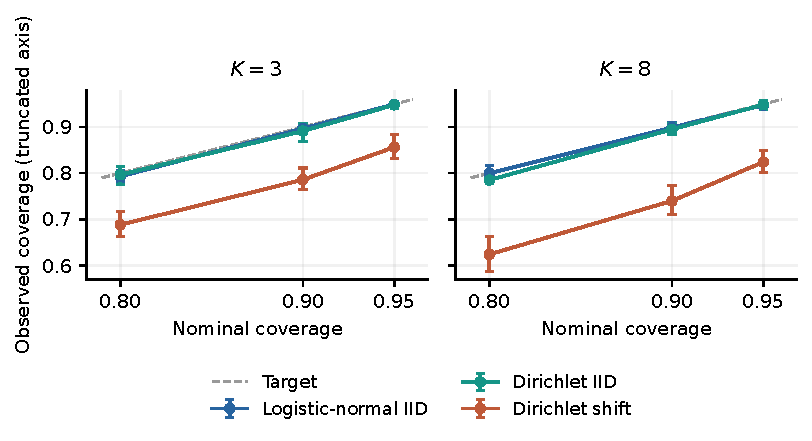
\includegraphics[width=.98\textwidth]{figures/coverage_by_regime.pdf}
\caption{Observed-composition coverage for scaled ILR. Left: $K=3$; right: $K=8$. Whiskers are descriptive 95\% seed-block bootstrap intervals derived from retained observations. The truncated vertical axis highlights departures from the dashed nominal-coverage reference. IID behavior is close to target; the shifted Dirichlet deficit is substantial at every level. Lines connect nominal levels, not time.}
\label{fig:coverage}
% @evidence[[analysis/summary.json#/coverage]]
\end{figure}

The shifted deficit is larger and consistent across levels. At nominal 0.90, mean coverage falls to 0.7858 [0.7647, 0.8112] for $K=3$ and 0.7399 [0.7096, 0.7739] for $K=8$. At nominal 0.80, the corresponding means are 0.6880 and 0.6239. Mean absolute error across seed-condition-level records increases from 0.0136 in IID conditions to 0.1303 under shift. This is evidence against interpreting training-only scale adaptation as a shift-robust calibration procedure. It is not evidence that conformal prediction failed under its exchangeability assumptions: those assumptions are absent in this test regime. % @evidence[[analysis/summary.json#/coverage]]
% @evidence[[paper_data.json#/final_evaluation/metrics]]

\subsection{Aggregate utility and simplex mass favor different readings}
Table~\ref{tab:main} reports all standard comparators. Scaled ILR has mean utility 0.6618, compared with 0.6502 for simplex max, 0.6296 for Bonferroni, and 0.6047 for unscaled ILR. Its paired aggregate utility advantage over simplex max is 0.0116 [0.0047, 0.0179]. Nevertheless, its mean simplex mass is 0.3035 rather than 0.2917 for simplex max. The favorable utility contrast therefore does not mean the scale-adaptive regions are smaller on average. % @evidence[[analysis/summary.json#/methods]]
% @evidence[[analysis/summary.json#/paired_overall]]

\begin{table}[t]
\centering\small
\caption{Held-out mean errors, normalized simplex mass, and utility. Errors are absolute deviations computed before averaging. Utility intervals are descriptive joint seed-block bootstrap intervals from our retained-data analysis. Smaller error and mass are favorable; larger utility is favorable.}
\label{tab:main}
\begin{tabular}{lrrrr}
\toprule
Method & IID error & Shift error & Mass & Utility [95\% interval] \\
\midrule
Scaled ILR & 0.0136 & 0.1303 & 0.3035 & 0.6618 [0.6542, 0.6702] \\
Unscaled ILR & 0.0114 & 0.2162 & 0.3382 & 0.6047 [0.5980, 0.6107] \\
Simplex max & 0.0112 & 0.1974 & 0.2917 & 0.6502 [0.6438, 0.6568] \\
Bonferroni & 0.0204 & 0.1620 & 0.3192 & 0.6296 [0.6223, 0.6367] \\
\bottomrule
\end{tabular}

% @evidence[[analysis/summary.json#/methods]]
\end{table}

The same table also prevents an overly favorable reliability interpretation. Both unscaled ILR and simplex max have slightly smaller aggregate IID errors than scaled ILR, whereas all three have larger shifted errors. Bonferroni has IID error 0.0204 and shifted error 0.1620. The scale-adaptive construction reduces aggregate mass relative to unscaled ILR, from 0.3382 to 0.3035, and improves utility by 0.0572 [0.0509, 0.0642]. This is evidence about the full scaling package at the common center, not a measured gain attributable specifically to rank selection. % @evidence[[analysis/summary.json#/methods]]
% @evidence[[analysis/summary.json#/paired_overall/unscaled_ilr]]

\subsection{Condition-specific comparisons rule out uniform dominance}
Figure~\ref{fig:paired} compares scaled ILR with simplex max. Positive utility differences and negative mass differences have different favorable directions, shown in separate columns. The largest favorable contrasts occur for IID Dirichlet responses at $K=8$. At $\alpha=0.10$, utility increases by 0.1962 [0.1741, 0.2168], while mass decreases by 0.2024 with interval [$-0.2254$,$-0.1800$]. All reported nominal levels in that condition favor scaled ILR on both quantities. This localized pattern is stronger than the small aggregate utility difference, but it does not identify which part of the scaling construction is responsible. % @evidence[[analysis/summary.json#/retained_uncertainty/DIR_IID_K8/paired_baselines/simplex_linf]]

\begin{figure}[t]
\centering
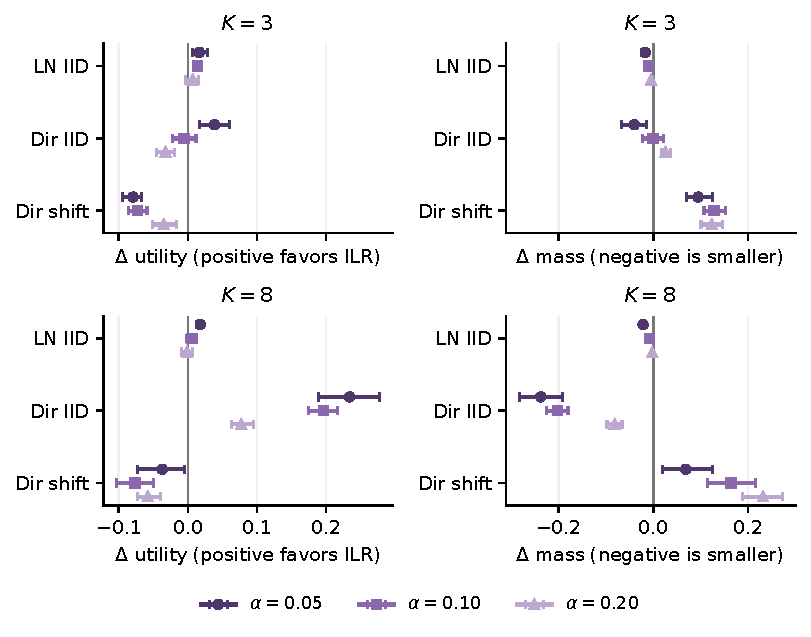
\includegraphics[width=.98\textwidth]{figures/paired_region_tradeoffs.pdf}
\caption{Scaled ILR minus simplex max, with evaluator-supplied paired descriptive 95\% seed-bootstrap intervals. Rows distinguish $K$; columns distinguish utility (positive favors scaled ILR) and uniform-simplex mass (negative means smaller). All nominal levels are shown. LN denotes logistic-normal; Dir denotes Dirichlet. Shifted conditions reverse the favorable IID Dirichlet pattern.}
\label{fig:paired}
% @evidence[[analysis/summary.json#/retained_uncertainty]]
\end{figure}

The contrasts are not uniformly favorable even without shift. For IID Dirichlet $K=3$ at $\alpha=0.20$, utility is lower by 0.0323 [$-0.0451$,$-0.0199$], and mass is larger by 0.0261. Several logistic-normal contrasts are small, with descriptive intervals including zero. These results reject a blanket preference for scaled ILR across response laws, dimensions, and target levels. % @evidence[[analysis/summary.json#/retained_uncertainty/DIR_IID_K3/paired_baselines/simplex_linf]]
% @evidence[[analysis/summary.json#/retained_uncertainty/LN_IID_K8/paired_baselines/simplex_linf]]

Every shifted utility contrast against simplex max is negative, and every shifted mass contrast is positive. At $\alpha=0.10$, utility differences are $-0.0732$ [$-0.0858$,$-0.0591$] for $K=3$ and $-0.0765$ [$-0.1032$,$-0.0492$] for $K=8$. Corresponding mass increases are 0.1281 and 0.1639. Importantly, scaled ILR still has the smaller aggregate shifted coverage error: its adverse shifted utility comparison cannot be summarized as worse coverage alone. The larger regions offset that reliability advantage under the supplied utility. % @evidence[[analysis/summary.json#/retained_uncertainty/DIR_SHIFT_K3/paired_baselines/simplex_linf]]
% @evidence[[analysis/summary.json#/retained_uncertainty/DIR_SHIFT_K8/paired_baselines/simplex_linf]]

\subsection{Controls and what they identify}
The evaluator checks reset behavior, constant inputs, permuted inputs, and a zero-radius point-copy control. All recorded checks pass. Constant-input and permuted-input comparisons disrupt access to predictive features at query time; they are information controls, not training-time component removals. Likewise, whole-simplex and zero-radius endpoints check the meaning of mass and coverage but cannot recommend a useful predictive region. Feature-group coverage by the sign of $x_0$ is reported in the supplement to expose heterogeneity without claiming groupwise calibration. No group-specific threshold is fitted. % @evidence[[paper_data.json#/final_evaluation/metrics/control_check_pass_rate]]
% @evidence[[paper_data.json#/final_evaluation/evaluation_evidence/episodes]]

\section{Discussion and Limitations}
\paragraph{What the positive comparisons establish.}
At the evaluated center and data budget, the scaling package can improve utility and reduce simplex mass relative to removing scaling. It also provides large paired gains against simplex max in the higher-dimensional IID Dirichlet condition. These are valid configuration-level comparisons, with matched data and reported seed variation. They are not evidence that every constituent is needed, nor that the rank-based objective is preferable to Gaussian-loss selection. The final measurements contain no matched selector-only comparison. Development configurations change multiple choices and use a different evidence split, so their scores cannot fill that gap.

\paragraph{Why the negative comparisons matter.}
The mismatch between the selection objective and the evaluation reference measure is an explicit limitation of the construction. The result is compatible with that mismatch, but does not isolate it as the cause of unfavorable mass differences. The shift also jointly changes support, feature frequencies, and the frequency of high-variability responses. Its adverse coverage cannot be attributed solely to extrapolation, scale misspecification, or one design choice without additional controlled evidence. Standard exchangeability theory explains why no unchanged guarantee is available, not the magnitude of the observed deficit.

\paragraph{Uncertainty and selection scope.}
Only the retained seed blocks quantify repetition. The audit framing is retrospective; its intervals do not adjust for choosing the manuscript's emphasis. Paired resampling respects dependence across conditions and nominal levels, but few independent blocks limit precision, especially at multiplicity-adjusted tails. Conditional-on-fit Wilson intervals, Monte Carlo mass diagnostics, and seed-bootstrap intervals answer different questions. Shared probes introduce dependence across contexts, so an average of per-context standard errors is not a confidence interval for the overall mass. The main comparisons and the overall utility gap are descriptive; no claim is made that they remain significant after arbitrary selection of endpoints or across unobserved tasks.

\paragraph{Domain and geometric scope.}
The study has no public-data experiment, alternative ILR basis, learned covariance region, structural-zero response, or independent boundary-face reference measure. Positivity flooring makes logratios computable but is not a principled solution for true zeros. Uniform-simplex mass is a clearly defined reference measure, not a universal notion of user-relevant uncertainty. Its dimension dependence and finite probe resolution can hide small or boundary-concentrated regions. Conversely, a smaller mass need not imply better prediction for the actual response law. These limitations prevent conclusions about classification label sets, latent probability regions, or general deployment reliability.

\paragraph{Practical interpretation.}
The evidence recommends an evaluation discipline rather than a universal method choice: specify the response being covered, state the reference measure, compare matched configurations, retain condition-specific failures, and distinguish marginal from conditional and shifted validity. Aggregate utility can be useful for summarization only after its components are visible. Where support changes or calibration is reused for selection, assumptions must be reassessed rather than inferred from an apparently favorable score. Neither issue is repaired by a publication decision or by satisfying a completion check.

\section{Conclusion}
Scale-adaptive conformal regions for continuous compositions exhibit a measurable but bounded reliability--efficiency trade-off. In the evaluated synthetic settings, independent split calibration gives near-target IID behavior, and the complete scaling construction improves aggregate utility relative to the unscaled matched-center alternative. Against the simplex-coordinate maximum-residual baseline, however, the positive aggregate utility difference coexists with larger overall simplex mass, favorable higher-dimensional IID Dirichlet comparisons, and adverse shifted comparisons. No uniformly superior region construction emerges from these measurements.

The distinction between training-time ILR-box volume and evaluation-time uniform-simplex mass is therefore essential to interpreting the method. Equally essential is the distinction between IID calibration and shifted reliability: training-only adaptation preserves the standard calibration argument but does not make it shift-invariant. Further evidence would be needed to isolate the selector's contribution, assess support-preserving shifts, or study structural zeros and real responses. Within the available evidence, the defensible conclusion is that coverage, geometric efficiency, and assumptions must be audited separately, with configuration-level gains stated at their measured scope.

\clearpage
\bibliography{references}
\bibliographystyle{iclr2026_conference}
\clearpage
\appendix
\section{Supplementary Information}
\label{sec:supplement}

\subsection{Detailed selection specification and algebraic checks}
The archived implementation is \texttt{source\_evidence/selected\_model.py}; the evaluated entrypoint declaration is retained in \texttt{source\_evidence/selected\_spec.toml}. Basis and design construction appear at lines 89--107; base fitting and moment tables at lines 114--152; smoothing and bounded scale correction at lines 154--185; Gaussian-loss fallback at lines 188--234; and rank-based selection at lines 237--352. These readable implementations, rather than a hash or a previous assessment, support the concrete method description. % @evidence[[source_evidence/selected_model.py]]

Each call to the deterministic fold constructor permutes the relevant training indices with NumPy random seed 0 and splits them into three parts. Feature standard deviations in moment tables are bounded below by $10^{-8}$, standardized residual scales by $10^{-4}$, and kernel queries are processed in batches of 128. Neutral settings share predictions even when their redundant bandwidth or prior parameters differ. The method caches moment-ratio evaluations for repeated bandwidth/prior pairs. The selector's outer pseudo-calibration halves and evaluation halves are disjoint from one another and from the rows fitting their models. Internal folds overlap across fits and must not be counted as independent scientific replications. % @evidence[[source_evidence/selected_model.py#_training_folds]]

To check global-scale invariance, replace $s(x)$ by $c\,s(x)$ for constant $c>0$, ignoring numerical clipping. Every calibration score is divided by $c$, so its order-statistic radius becomes $q_\alpha/c$. The resulting coordinate half-width is $(q_\alpha/c)(c\,s_j(x))=q_\alpha s_j(x)$. Its ILR-box volume is unchanged:
\begin{equation}
 (2q_\alpha/c)^{K-1}\prod_{j=1}^{K-1}c\,s_j(x)
 =(2q_\alpha)^{K-1}\prod_{j=1}^{K-1}s_j(x).
\end{equation}
The source includes a numerical assertion for this cancellation away from clipping bounds. This is an algebraic implementation check, not an independently measured ablation. For the inner rank rule at $\alpha=0.05$, 18 pseudo-calibration observations cannot give a finite rank while 19 can. A zero radius is rejected by the selector, although a zero threshold is meaningful for the evaluator's deliberately degenerate point control. No realized fallback count is available. % @evidence[[source_evidence/selected_model.py#_assert_rank_selection_controls]]

\subsection{Generator, target, and reproducibility specification}
The generator is archived in \texttt{source\_evidence/evaluate\_final.py}, lines 701--760. With zero-based indices, $W_{\ell j}=\sin(\ell(K-1)+j+1)/3$, $\ell=0,\ldots,5$. In the Helmert basis, column $j-1$ has its first $j$ entries $1/\sqrt{j(j+1)}$, entry $j$ equal to $-j/\sqrt{j(j+1)}$, and remaining entries zero. These conventions fix both the generated response and the fitted-coordinate interpretation. % @evidence[[source_evidence/evaluate_final.py#basis]]

Training, calibration, test, and reference-probe random streams are separated using \texttt{SeedSequence([seed, case\_index, split\_index, 202611])}; the reference stream has split index 3. The manifest stores array and row provenance and the evaluator checks normalized float64 hashes, positive responses, closure, feature shapes, and split-content disjointness. The retained manifest is \texttt{source\_evidence/data\_manifest.json}; hashes identify the retained data but do not establish substantive methodological properties. The response is always the observed continuous vector; no latent target or categorical observation is substituted. % @evidence[[source_evidence/evaluate_final.py#load_resources]]

\textbf{Environment and commands.} The evaluated implementation requires CPython 3.11 or 3.12 and NumPy 1.26.4, uses CPU computation, and has no downloaded dataset, pretrained model, or external data license requirement. The native evaluator additionally requires Linux process-isolation facilities documented in \texttt{source\_evidence/task\_contract.json}; a portable re-execution should not silently bypass those controls. \texttt{REPRODUCIBILITY.md} records the evaluator command, complete retained-data analysis commands, and artifact mappings. The plotting environment used here is recorded separately in \texttt{analysis/environment.json}; it is not represented as the historical evaluation environment. Runtime is not estimated from plotting time, and the final evaluation was not rerun during manuscript preparation. % @evidence[[source_evidence/requirements.txt]]
% @evidence[[source_evidence/task_contract.json]]
% @evidence[[analysis/environment.json]]

\subsection{Complete condition-level results and paired comparisons}
The following tables retain every condition, nominal level, and standard baseline. Utility and mass differences are always scaled ILR minus the named comparator. The 95\% paired intervals and adjusted utility endpoints are copied from the deduplicated evaluator uncertainty record, while the coverage intervals are newly derived from existing seed-level observations. Adjusted utility endpoints do not apply to mass or feature-group coverage. Rounding is for display only; machine-readable values remain in \texttt{analysis/summary.json}. % @evidence[[analysis/summary.json]]
% Embedded from analysis/coverage_table.tex; regenerate with build_analysis.py.
\begin{table}[p]
\centering\small
\caption{Scaled-ILR results by condition. Coverage intervals resample seed blocks; mass and utility are empirical means.}
\begin{tabular}{llrrrr}
\toprule
Condition & $\alpha$ & Coverage & 95\% interval & Mass & Utility \\
\midrule
LN K3 & 0.05 & 0.9491 & [0.9432,0.9558] & 0.1308 & 0.8620 \\
LN K3 & 0.10 & 0.8965 & [0.8906,0.9020] & 0.0976 & 0.8955 \\
LN K3 & 0.20 & 0.7930 & [0.7815,0.8054] & 0.0676 & 0.9127 \\
LN K8 & 0.05 & 0.9475 & [0.9407,0.9555] & 0.0035 & 0.9874 \\
LN K8 & 0.10 & 0.8986 & [0.8882,0.9106] & 0.0018 & 0.9829 \\
LN K8 & 0.20 & 0.7997 & [0.7852,0.8162] & 0.0009 & 0.9748 \\
Dir K3 & 0.05 & 0.9481 & [0.9396,0.9541] & 0.3980 & 0.5977 \\
Dir K3 & 0.10 & 0.8912 & [0.8693,0.9072] & 0.3141 & 0.6707 \\
Dir K3 & 0.20 & 0.7967 & [0.7758,0.8149] & 0.2324 & 0.7473 \\
Dir K8 & 0.05 & 0.9485 & [0.9387,0.9572] & 0.5627 & 0.4320 \\
Dir K8 & 0.10 & 0.8951 & [0.8841,0.9072] & 0.4462 & 0.5441 \\
Dir K8 & 0.20 & 0.7850 & [0.7773,0.7927] & 0.3165 & 0.6703 \\
Shift K3 & 0.05 & 0.8563 & [0.8323,0.8832] & 0.4909 & 0.4577 \\
Shift K3 & 0.10 & 0.7858 & [0.7647,0.8112] & 0.4042 & 0.5192 \\
Shift K3 & 0.20 & 0.6880 & [0.6633,0.7163] & 0.3142 & 0.5885 \\
Shift K8 & 0.05 & 0.8240 & [0.8009,0.8492] & 0.6622 & 0.2920 \\
Shift K8 & 0.10 & 0.7399 & [0.7096,0.7739] & 0.5668 & 0.3540 \\
Shift K8 & 0.20 & 0.6239 & [0.5877,0.6634] & 0.4528 & 0.4238 \\
\bottomrule
\end{tabular}
\end{table}
% Embedded from analysis/complete_comparisons.tex; regenerate with build_analysis.py.
\begin{table}[p]
\centering\scriptsize
\caption{Scaled ILR minus Unscaled ILR. Descriptive paired 95\% intervals and adjusted utility endpoints are supplied by the evaluator. Mass intervals are unadjusted.}
\begin{tabular}{llrrrrr}
\toprule
Condition & $\alpha$ & $\Delta U$ & 95\% interval & Adjusted interval & $\Delta M$ & 95\% interval \\
\midrule
LN K3 & 0.05 & -0.003 & [-0.007,+0.002] & [-0.009,+0.006] & +0.002 & [-0.001,+0.005] \\
LN K3 & 0.10 & -0.005 & [-0.009,-0.001] & [-0.011,+0.002] & +0.003 & [+0.000,+0.005] \\
LN K3 & 0.20 & -0.006 & [-0.012,+0.001] & [-0.016,+0.005] & +0.001 & [+0.000,+0.001] \\
LN K8 & 0.05 & +0.001 & [-0.003,+0.006] & [-0.006,+0.010] & +0.001 & [+0.000,+0.001] \\
LN K8 & 0.10 & +0.001 & [-0.008,+0.010] & [-0.012,+0.017] & +0.000 & [+0.000,+0.000] \\
LN K8 & 0.20 & +0.004 & [-0.009,+0.018] & [-0.016,+0.027] & +0.000 & [+0.000,+0.000] \\
Dir K3 & 0.05 & +0.119 & [+0.094,+0.145] & [+0.081,+0.159] & -0.117 & [-0.141,-0.096] \\
Dir K3 & 0.10 & +0.031 & [+0.018,+0.043] & [+0.010,+0.050] & -0.041 & [-0.056,-0.026] \\
Dir K3 & 0.20 & -0.026 & [-0.036,-0.015] & [-0.040,-0.008] & +0.019 & [+0.009,+0.029] \\
Dir K8 & 0.05 & +0.367 & [+0.334,+0.406] & [+0.323,+0.433] & -0.372 & [-0.413,-0.337] \\
Dir K8 & 0.10 & +0.300 & [+0.287,+0.315] & [+0.280,+0.326] & -0.306 & [-0.325,-0.289] \\
Dir K8 & 0.20 & +0.107 & [+0.100,+0.115] & [+0.095,+0.119] & -0.111 & [-0.123,-0.098] \\
Shift K3 & 0.05 & -0.025 & [-0.046,-0.005] & [-0.059,+0.007] & +0.052 & [+0.019,+0.088] \\
Shift K3 & 0.10 & -0.033 & [-0.043,-0.021] & [-0.050,-0.014] & +0.100 & [+0.078,+0.124] \\
Shift K3 & 0.20 & +0.016 & [-0.004,+0.034] & [-0.020,+0.044] & +0.129 & [+0.110,+0.150] \\
Shift K8 & 0.05 & +0.139 & [+0.106,+0.179] & [+0.095,+0.203] & -0.148 & [-0.200,-0.106] \\
Shift K8 & 0.10 & +0.049 & [+0.020,+0.088] & [+0.010,+0.121] & -0.008 & [-0.064,+0.040] \\
Shift K8 & 0.20 & -0.007 & [-0.024,+0.019] & [-0.028,+0.041] & +0.172 & [+0.108,+0.226] \\
\bottomrule
\end{tabular}
\end{table}
\begin{table}[p]
\centering\scriptsize
\caption{Scaled ILR minus Simplex max. Descriptive paired 95\% intervals and adjusted utility endpoints are supplied by the evaluator. Mass intervals are unadjusted.}
\begin{tabular}{llrrrrr}
\toprule
Condition & $\alpha$ & $\Delta U$ & 95\% interval & Adjusted interval & $\Delta M$ & 95\% interval \\
\midrule
LN K3 & 0.05 & +0.017 & [+0.006,+0.028] & [+0.003,+0.036] & -0.017 & [-0.025,-0.010] \\
LN K3 & 0.10 & +0.014 & [+0.009,+0.019] & [+0.005,+0.022] & -0.010 & [-0.014,-0.005] \\
LN K3 & 0.20 & +0.007 & [-0.003,+0.015] & [-0.009,+0.019] & -0.004 & [-0.007,-0.002] \\
LN K8 & 0.05 & +0.018 & [+0.012,+0.022] & [+0.008,+0.024] & -0.021 & [-0.024,-0.019] \\
LN K8 & 0.10 & +0.006 & [-0.001,+0.012] & [-0.008,+0.015] & -0.007 & [-0.009,-0.006] \\
LN K8 & 0.20 & -0.001 & [-0.010,+0.007] & [-0.015,+0.012] & -0.002 & [-0.003,-0.002] \\
Dir K3 & 0.05 & +0.038 & [+0.017,+0.061] & [+0.004,+0.074] & -0.040 & [-0.066,-0.015] \\
Dir K3 & 0.10 & -0.006 & [-0.022,+0.012] & [-0.032,+0.022] & -0.001 & [-0.023,+0.022] \\
Dir K3 & 0.20 & -0.032 & [-0.045,-0.020] & [-0.053,-0.013] & +0.026 & [+0.017,+0.036] \\
Dir K8 & 0.05 & +0.234 & [+0.189,+0.278] & [+0.159,+0.303] & -0.237 & [-0.283,-0.192] \\
Dir K8 & 0.10 & +0.196 & [+0.174,+0.217] & [+0.158,+0.229] & -0.202 & [-0.225,-0.180] \\
Dir K8 & 0.20 & +0.077 & [+0.062,+0.094] & [+0.056,+0.104] & -0.082 & [-0.098,-0.066] \\
Shift K3 & 0.05 & -0.079 & [-0.094,-0.067] & [-0.104,-0.063] & +0.095 & [+0.071,+0.125] \\
Shift K3 & 0.10 & -0.073 & [-0.086,-0.059] & [-0.090,-0.049] & +0.128 & [+0.107,+0.152] \\
Shift K3 & 0.20 & -0.035 & [-0.052,-0.016] & [-0.059,-0.003] & +0.124 & [+0.101,+0.147] \\
Shift K8 & 0.05 & -0.037 & [-0.073,-0.004] & [-0.096,+0.012] & +0.068 & [+0.019,+0.124] \\
Shift K8 & 0.10 & -0.077 & [-0.103,-0.049] & [-0.118,-0.031] & +0.164 & [+0.114,+0.216] \\
Shift K8 & 0.20 & -0.058 & [-0.074,-0.040] & [-0.081,-0.025] & +0.232 & [+0.189,+0.273] \\
\bottomrule
\end{tabular}
\end{table}
\begin{table}[p]
\centering\scriptsize
\caption{Scaled ILR minus Bonferroni. Descriptive paired 95\% intervals and adjusted utility endpoints are supplied by the evaluator. Mass intervals are unadjusted.}
\begin{tabular}{llrrrrr}
\toprule
Condition & $\alpha$ & $\Delta U$ & 95\% interval & Adjusted interval & $\Delta M$ & 95\% interval \\
\midrule
LN K3 & 0.05 & +0.031 & [+0.021,+0.043] & [+0.018,+0.050] & -0.027 & [-0.034,-0.021] \\
LN K3 & 0.10 & +0.029 & [+0.023,+0.038] & [+0.021,+0.046] & -0.021 & [-0.026,-0.016] \\
LN K3 & 0.20 & +0.046 & [+0.027,+0.066] & [+0.016,+0.077] & -0.018 & [-0.022,-0.014] \\
LN K8 & 0.05 & +0.026 & [+0.021,+0.032] & [+0.018,+0.036] & -0.026 & [-0.031,-0.021] \\
LN K8 & 0.10 & +0.007 & [-0.004,+0.018] & [-0.013,+0.023] & -0.010 & [-0.012,-0.008] \\
LN K8 & 0.20 & +0.015 & [+0.006,+0.025] & [+0.002,+0.031] & -0.003 & [-0.004,-0.003] \\
Dir K3 & 0.05 & +0.087 & [+0.064,+0.106] & [+0.047,+0.115] & -0.085 & [-0.101,-0.064] \\
Dir K3 & 0.10 & +0.043 & [+0.022,+0.064] & [+0.011,+0.078] & -0.044 & [-0.063,-0.027] \\
Dir K3 & 0.20 & +0.042 & [+0.024,+0.057] & [+0.012,+0.066] & -0.018 & [-0.027,-0.008] \\
Dir K8 & 0.05 & +0.246 & [+0.207,+0.285] & [+0.182,+0.308] & -0.250 & [-0.291,-0.211] \\
Dir K8 & 0.10 & +0.216 & [+0.192,+0.242] & [+0.178,+0.259] & -0.222 & [-0.250,-0.197] \\
Dir K8 & 0.20 & +0.146 & [+0.131,+0.160] & [+0.118,+0.169] & -0.139 & [-0.155,-0.126] \\
Shift K3 & 0.05 & -0.055 & [-0.074,-0.040] & [-0.088,-0.035] & +0.051 & [+0.019,+0.092] \\
Shift K3 & 0.10 & -0.072 & [-0.085,-0.058] & [-0.092,-0.047] & +0.084 & [+0.060,+0.109] \\
Shift K3 & 0.20 & -0.064 & [-0.081,-0.046] & [-0.088,-0.033] & +0.084 & [+0.059,+0.108] \\
Shift K8 & 0.05 & -0.023 & [-0.060,+0.009] & [-0.083,+0.020] & +0.047 & [-0.004,+0.104] \\
Shift K8 & 0.10 & -0.066 & [-0.092,-0.040] & [-0.106,-0.022] & +0.130 & [+0.081,+0.184] \\
Shift K8 & 0.20 & -0.073 & [-0.088,-0.055] & [-0.094,-0.040] & +0.186 & [+0.140,+0.230] \\
\bottomrule
\end{tabular}
\end{table}

\subsection{Feature-group reliability and information controls}
The two observable audit groups are $x_0>0$ and $x_0\leq0$. They are defined by an input, not by a realized response, and do not create group-specific calibration thresholds. Figure~\ref{fig:groups} reports mean group coverage at nominal 0.90, with joint seed-block intervals. Each seed contributes its group fraction, rather than pooling all test rows as independent repeated fits. Group sample counts and per-seed Wilson intervals are retained in the final evidence. The visual comparison is descriptive and not a test of full conditional validity. % @evidence[[analysis/summary.json#/feature_groups_alpha_010]]

\begin{figure}[ht]
\centering
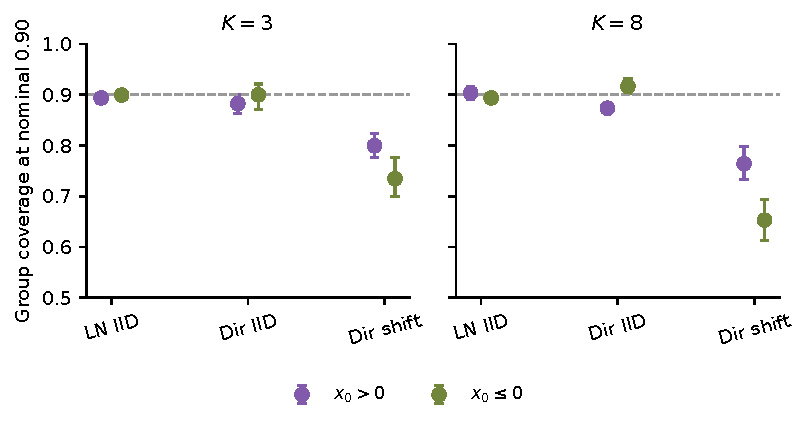
\includegraphics[width=.98\textwidth]{figures/feature_group_reliability.pdf}
\caption{Feature-group coverage of scaled ILR at nominal 0.90. Whiskers are descriptive seed-block 95\% bootstrap intervals; the dashed line marks the target, not a groupwise guarantee. Both dimensions retain the shifted reliability deficit. These audit groups are not used for Mondrian calibration.}
\label{fig:groups}
% @evidence[[analysis/summary.json#/feature_groups_alpha_010]]
\end{figure}

The constant-input control replaces each query feature vector by the training-feature mean before prediction. The permuted-input control rotates calibration rows and test rows separately, disrupting feature-response alignment without transferring labels. The constant-center reference uses the training mean in ILR coordinates and unit scales. These controls change information available at prediction time or the center itself; they are not interchangeable with the matched-center unscaled comparison. The evaluator supplies feature-control paired utility intervals in the retained uncertainty object. We do not use passing controls as evidence that every scientific validity threat has been excluded. % @evidence[[source_evidence/evaluate_final.py#evaluate_episode]]

\subsection{Reference-mass resolution and degenerate controls}
Uniform-simplex probes are shared across test contexts and methods within each condition/seed. The per-context reported standard-error diagnostic is $\sqrt{\widehat p(1-\widehat p)/1024}$; the evaluator averages this diagnostic across contexts. It is not a valid replacement for a joint uncertainty calculation because the same probes are reused. At zero hits, the plugin diagnostic vanishes even though the one-sided binomial upper bound is positive. Reporting a zero mass estimate must therefore not be converted into a claim of zero geometric volume. This distinction is especially relevant for small high-dimensional regions. % @evidence[[source_evidence/evaluate_final.py#method_records]]

The whole-simplex construction has unit reference mass and covers every observed composition; its utility is zero because the efficiency factor vanishes. The zero-radius reference tests equality with a fitted point, not recovery of the original observation. These endpoints check that metric behavior is interpretable, but do not supply an efficiency comparison among useful calibrated sets. No separate integration over simplex faces or boundary strata is present. All measured mass refers to the full-dimensional uniform-simplex reference distribution. % @evidence[[source_evidence/evaluate_final.py#method_records]]

\subsection{Evidence provenance and comparison scope}
The independent final record reports completion, qualification, and successful specified checks. Qualification facts are grounded in the final qualification fields, independently of any development summary; they do not strengthen the statistical claims. The manuscript retains the shifted deficits and unfavorable region-size comparisons despite that outcome. The original initializer has no matched held-out result in this bundle, so no final comparison with it is reported. % @evidence[[paper_data.json#/final_evaluation/status]]
% @evidence[[paper_data.json#/final_evaluation/outcome]]
% @evidence[[paper_data.json#/final_evaluation/correct]]

Development evidence also contains a joint center/scale configuration and a Gaussian-selected local-moment configuration, archived in \texttt{source\_evidence/development\_joint.py} (line 152) and \texttt{source\_evidence/development\_gaussian.py} (line 185). They are provenance context, not final selector ablations: their scores are development measurements, not held-out measurements of the same controlled intervention. The main text consequently reports neither development-score margins nor a selector-specific causal advantage. Proposed alternative geometries, groupwise calibration, and latent-target diagnostics are not treated as completed measurements. Missing experiments remain limitations, not negative outcomes. % @evidence[[paper_data.json#/all_programs]]

\subsection{LLM Usage}
Language models assisted hypothesis formulation, training-only method design, implementation preparation, reference-query planning, synthesis of retained measurements, manuscript drafting, and construction of plotting and validation scripts. The manuscript-writing assistant inspected archived implementations and final records, generated figures from existing measurements, and retrieved exact foundational references for the cited background. It did not generate new scientific evaluation episodes. The overview figure is prepared through an automated concept-figure workflow; quantitative plots are deterministic visualizations of retained records. No model-generated number is used as an empirical result. No human-supervision procedure or independent replication is asserted beyond the documented checks. The process logs are retained for audit without identifying authors.

\end{document}
